\clearpage
\phantomsection

\setcounter{chapter}{2}
\chapter[NHẬN DẠNG HỆ THỐNG SỬ DỤNG MẠNG HỌC SÂU]{Nhận dạng hệ thống sử dụng mạng học sâu}
\label{sec:ML}

Trong chương này, tác giả sẽ đề xuất một mô hình mạng học sâu ISD sử dụng cho nhận dạng hệ thống viễn thông MIMO/mMIMO. Đầu tiên, sơ lược về hai hướng tiếp cận sử dụng mạng nơ-ron học sâu sẽ được giới thiệu, trong đó chi tiết về mô hình mạng DetNet được trình bày để so sánh trong các kết quả mô phỏng. Tiếp đến, từ một mô hình mạng ISD đã được đề xuất trong~\cite{Mandloi2017}, kết hợp với cách tiếp cận của mạng DNN tại~\cite{Liao2020}, tác giả sẽ đề xuất một mạng học sâu ISD cải tiến để nhận dạng hệ thống. Các bước mô phỏng và đánh giá sẽ được đưa ra để cho thấy tiềm năng của phương pháp đề xuất và đưa ra kết luận của chương. 

\section{Giới thiệu về mạng nơ-ron học sâu DetNet}

Trong chương~\ref{sec:back}, các phương pháp nhận dạng hệ thống sử dụng các phương pháp ML/DL đã được chia làm ba loại, trong đó phương pháp sử dụng các mạng nơ-ron đang được quan tâm nghiên cứu. Các mạng nơ-ron sâu (DNN - Deep-neural network) đã được sử rụng rộng rãi trong các ứng dụng như xử lý tiếng nói, ngôn ngữ tự nhiên, hình ảnh, thị giác máy, trò chơi trực tuyến~\cite{Samek2021}. Mười năm trở lại đây, nhiều nghiên cứu ứng dụng các mô hình mạng DNN khác nhau cho nhận dạng hệ thống viễn thông không dây. Có thể chia các phương pháp này thành hai kiểu chính, bao gồm hướng dữ liệu (data-driven) và hướng mô hình (model-driven)~\cite{Liao2020}. Các phương pháp data-driven trực tiếp học các đặc trưng từ một tập lớn các dữ liệu (dataset) để phục vụ cho các mục đích như ước lượng kênh truyền, phản hồi CSI,~\ldots. Tuy các phương pháp data-driven được đề xuất đều cho độ chính xác cao nhưng vẫn có những thách thức khi yêu cầu số lượng mẫu rất lớn và kéo theo đó là thời gian cho việc đào tạo lâu. Các phương pháp model-driven~\cite{He2019} có thể một phần khắc phục các hạn chế này bằng việc tối ưu/đưa thêm các tham số học bằng DL vào các một hình có sẵn để kết hợp ưu điểm của data-driven và các mô hình toán học truyền thống. Trong số các phương pháp data-driven, mô hình mạng nơ-ron sâu DetNet sẽ được trình bày ngắn gọn dưới đây do trong mô hình đề xuất có một phần ý tưởng xuất phát từ mạng DNN DetNet.

Xét hệ thống MIMO/mMIMO tương tự đã trình bày ở hình~\ref{fig:sys_model}. Tuy nhiên, thay vì mô hình hoá tín kênh truyền vô tuyến dưới dạng các bộ lọc FIR có chiều dài $M+1$, trong DNN, giả sử: (i) $T$ có thể coi là số lượng ăng-ten bên phát hoặc số lượng người dùng (user) với mỗi người dùng chỉ có một ăng-ten phát, (ii) ma trận $\mathbf{H}$ là biến đổi tuyến tính của tín hiệu truyền thành tín hiệu nhận được, (iii) $N=1$ tức mỗi ăng-ten nhận chỉ thu thập một ký hiệu tại một thời điểm, (iv) các ma trận sẽ được chuyển đổi sang dạng phần thực, ảo riêng biệt như phương trình (\ref{eq:matrixtras1}) và (\ref{eq:matrixtras2}). Biểu diễn đơn giản cho hệ thống MIMO/mMIMO như sau
\begin{equation}
    \mathbf{x} = \mathbf{H} \mathbf{s} + \mathbf{w}
\end{equation}
trong đó, $\mathbf{H} \in \mathbb{R}^{2L \times 2T}$, $\mathbf{s} \in \mathbb{R}^{2T \times 1}$, $\mathbf{w} \in \mathbb{R}^{2L \times 1}$, và $\mathbf{x} \in \mathbb{R}^{2L \times 1}$. Để tìm bộ nhận dạng cho hệ thống kể trên, định nghĩa hàm mất mát $l\left(\mathbf{s} ; \hat{\mathbf{s}}_{\boldsymbol{\theta}}(\mathbf{H}, \mathbf{x})\right)$ là khoảng cách giữa ký hiệu gốc và ký hiệu được ước lượng. Tìm giá trị $\mathbf{\theta}$ bằng cách tối thiểu hoá hàm mất mát kể trên  
\begin{equation}
\label{eq:lossf}
\min _{\boldsymbol{\theta}} \mathbb{E}\left\{l\left(\mathbf{s} ; \hat{\mathbf{s}}_{\boldsymbol{\theta}}(\mathbf{H}, \mathbf{x})\right)\right\}
\end{equation}

Giải thuật cho độ chính xác cao nhất để giải quyết (\ref{eq:lossf}) là bộ ước lượng hợp lẽ cực đại (MLE - Maximum likelihood estimator) như sau
\begin{equation}
\label{eq:mle}
\hat{\mathbf{s}}_{\boldsymbol{\theta}}(\mathbf{x}, \mathbf{H})=\arg \min _{\mathbf{s} \in \mathbb{R}^{2T}}\|\mathbf{x}-\mathbf{H} \mathbf{s}\|^2
\end{equation}
Tuy nhiên, độ phức tạp của MLE sẽ tăng theo cấp số mũ $\mathcal{O}(2^T)$ nên khó để triển khai trong các hệ mMIMO. Do vậy, DetNet là phương pháp đề xuất nhằm đạt được tiệm cận độ chính xác với MLE. Trong nghiên cứu gốc, thay vì tạo ra một mạng nơ-ron nhằm ánh xạ trực tiếp từ $\mathbf{x}$ về $\mathbf{s}$, việc phân tách $\mathbf{x}$ thành các thành phần $\mathbf{H}, \mathbf{s},$ và $\mathbf{w}$ sẽ hiệu quả hơn
\begin{equation}
    \mathbf{H}^\top \mathbf{x}=\mathbf{H}^\top \mathbf{H s}+\mathbf{H}^\top \mathbf{w}
\end{equation}

Kiến trúc DetNet dựa trên phương pháp giảm độ dốc dựa kiến (projected gradient descent)~\cite{Chen2015} cho việc tối ưu MLE như trên (\ref{eq:mle}). Đạo hàm riêng được tách như trên (\ref{eq:pgd}) sử dụng luật chuỗi (chain rule)~\cite{Minka2000}.
\begin{equation}
\label{eq:pgd}
    \begin{aligned}
    \hat{\mathbf{s}}_{k+1} & =\Pi\left[\hat{\mathbf{s}}_k-\left.\delta_k \frac{\partial\|\mathbf{x}-\mathbf{H} \mathbf{s}\|^2}{\partial \mathbf{s}}\right|_{\mathbf{s}=\hat{\mathbf{s}}_k}\right] \\
    & =\Pi\left[\hat{\mathbf{s}}_k-\delta_k \mathbf{H}^\top \mathbf{x}+\delta_k \mathbf{H}^\top \mathbf{H} \hat{\mathbf{s}}_k\right]
    \end{aligned}
\end{equation}
với $\mathbf{s}_k$ là giá trị ước lượng tại lớp thứ $k$, $\Pi [.]$ là một phép chiếu phi tuyến tính, và $\delta_k$ là độ dài bước (step size) của quá trình học. Kiến trúc của mạng DetNet đề xuất trong~\cite{Samuel2017} được biểu biến như trên hình~\ref{fig:detnet} và cách biểu diễn dưới dạng ma trận như sau
\allowdisplaybreaks
\begin{subequations}
\begin{alignat}{4}
    \mathbf{z}_k & =\rho\left(\mathbf{W}_{1 k}\left[\begin{array}{c}
    \mathbf{H}^\top \mathbf{x} \\
    \hat{\mathbf{s}}_k \\
    \mathbf{H}^\top \mathbf{H} \hat{\mathbf{s}}_k \\
    \mathbf{v}_k
    \end{array}\right]+\mathbf{b}_{1 k}\right) \\
    \hat{\mathbf{s}}_{k+1} & =\psi_{t_k}\left(\mathbf{W}_{2 k} \mathbf{z}_k+ \mathbf{b}_{2 k}\right) \\
    \hat{\mathbf{v}}_{k+1} & =\mathbf{W}_{3 k} \mathbf{z}_k+ 
    \mathbf{b}_{3 k} \\
    \hat{\mathbf{s}}_1 & =\mathbf{0}
\end{alignat}
\end{subequations}
trong đó, $k = 1, \ldots, K$ là số các lớp của mạng DetNet, $\rho$ là một toán tử tuyến tính như ReLu hoặc Tanh. $\psi_{t_k}$ ký hiệu cho hàm tuyến tính phân đoạn, ở các mức $t$ khác nhau, $\psi_{t_k}(s)$ được minh hoạ trên hình~\ref{fig:soft_sign} và có biểu diễn toán học như sau
\begin{equation}
    \psi_{t_k}(s)=-1+\frac{\rho\left(s + t_k \right)}{\left|t_k\right|}-\frac{\rho\left(s- t_k \right)}{\left|t_k\right|}
\end{equation}

\begin{figure}[tb]
    \centering
    \begin{tikzpicture}
        \node (B11) [field6, fill=red!10!white] at (0, 0) {$\mathbf{H}^\top \mathbf{x}$};
        \node (B21) [below=10mm of B11, field6, fill=red!10!white] {$\mathbf{v}_k$};
        \node (B31) [below=10mm of B21, field6, fill=red!10!white] {$\mathbf{s}_k$};
        \node (B41) [below=10mm of B31, field6, fill=red!10!white] {$\mathbf{H}^\top \mathbf{H}$};

        
        \node (B32) [right=10mm of B31.south east, anchor=north, circle, fill=blue!10!white, draw=black] {$\times$}; 
        \node (B22) [right=25mm of B21, circle, fill=blue!10!white, draw=black] {$\operatorname{con}$};
        \node (B33) [below=11mm of B22, circle, fill=blue!10!white, draw=black] {$\times$};
        \node (B34) [below=4mm of B33, field8, fill=green!10!white, draw=black] {$\mathbf{W}_{1k}$};
        \node (B35) [right=7mm of B33, circle, fill=blue!10!white, draw=black] {$+$};
        \node (B36) [below=4mm of B35, field8, fill=green!10!white, draw=black] {$\mathbf{b}_{1k}$};

        \node (B37) [circle, fill=blue!10!white, draw=black] at (70mm, -30mm) {$\rho$};
        \node (B38) [right=40mm of B33, circle, fill=blue!10!white, draw=black] {$\times$};
        \node (B39) [below=4mm of B38, field8, fill=green!10!white, draw=black] {$\mathbf{W}_{2k}$};
        \node (B310) [right=7mm of B38, circle, fill=blue!10!white, draw=black] {$+$};
        \node (B311) [below=4mm of B310, field8, fill=green!10!white, draw=black] {$\mathbf{b}_{2k}$};
        \node (B312) [right=7mm of B310, circle, fill=blue!10!white, draw=black] {$\Psi$};

        \node (B23) [above=24.2mm of B39, circle, fill=blue!10!white, draw=black] {$\times$};
        \node (B24) [right=7mm of B23, circle, fill=blue!10!white, draw=black] {$+$};
        \node (B25) [above=4mm of B23, field8, fill=green!10!white, draw=black] {$\mathbf{W}_{3k}$};
        \node (B26) [above=4mm of B24, field8, fill=green!10!white, draw=black] {$\mathbf{b}_{3k}$};

        \node (Bvk1) [right=123mm of B21, field6, fill=red!10!white] {$\mathbf{v}_{k+1}$};
        \node (Bxk1) [right=123mm of B31, field6, fill=red!10!white] {$\mathbf{s}_{k+1}$};

        \draw[arrow] (B312) -- (Bxk1);
        \draw[arrow] (B24) -- (Bvk1);
        \draw[arrow] (B310) -- (B312);
        \draw[arrow] (B38) -- (B310);
        \draw[arrow] (B23) -- (B24);
        \draw[arrow] (B25) -- (B23);
        \draw[arrow] (B26) -- (B24);
        \draw[arrow] (B311) -- (B310);
        \draw[arrow] (B39) -- (B38);
        \draw[arrow] (B33) -- (B35);
        \draw[arrow] (B36) -- (B35);
        \draw[arrow] (B34) -- (B33);
        \draw[arrow] (B22) -- (B33);

        \draw[arrow] (B21) -- (B22);
        \draw[line] (B11) -- ([yshift=-3mm]B11.south);
        \draw[arrow] ([yshift=-3mm]B11.south) -| (B22);
        \draw[line] (B31) -- ([xshift=3mm]B31.east);
        \draw[arrow] ([xshift=3mm]B31.east) |- ([yshift=-1.5mm]B22.west);
        \draw[line] (B32) -- ([xshift=3mm]B32.east);
        \draw[arrow] ([xshift=3mm]B32.east) |- ([yshift=-3mm]B22.west);

        \draw[arrow] (B31) |- ([yshift=3mm]B32);
        \draw[arrow] (B41) |- ([yshift=-3mm]B32);

        \draw[arrow] (B37) |- (B38);
        \draw[arrow] (B37) |- (B23);
        \draw[arrow] (B35) |- (B37);
        
        \draw[arrow] (B41) -- (150mm, -60mm);
        \draw[arrow] (Bvk1) -- (150mm, -20mm);
        \draw[arrow] (Bxk1) -- (150mm, -41mm);
        \draw[arrow] (B11) -- (150mm, 0mm);

        % Legends
        \node[rectangle, draw=black, dashed, fill=black!5!white, minimum width=140mm, minimum height=35mm] at (70mm, -85mm) {};

        \node (B51) [field6, fill=red!10!white] at (22mm, -78mm) {Giá trị \\đầu vào/đầu ra};

        \node (B61) [below=4mm of B51, field8, fill=green!10!white, draw=black] {Giá trị học};

        \node (B52) [right=7mm of B51, circle, fill=blue!10!white, draw=black] {$\times$};
        \draw[arrow] (B52) -- ([xshift=3mm]B52.east) node [pos=0, right=3mm] {Nhân};

        \node (B53) [below=7mm of B52, circle, fill=blue!10!white, draw=black] {$+$};
        \draw[arrow] (B53) -- ([xshift=3mm]B53.east) node [pos=0, right=3mm] {Cộng};

        \node (B54) [right=20mm of B52, circle, fill=blue!10!white, draw=black] {$\rho$};
        \draw[arrow] (B54) -- ([xshift=10mm]B54.east) node [pos=0, right=10mm, above, label={below}:{tuyến tính}] {Toán tử};

        \node (B55) [right=20mm of B53, circle, fill=blue!10!white, draw=black] {$\Psi$};
        \draw[arrow] (B55) -- ([xshift=10mm]B55.east) node [pos=0, right=11mm, above, label={below}:{phi tuyến tính}] {Toán tử};

        \node (B56) [right=28mm of B54, circle, fill=blue!10!white, draw=black] {$\operatorname{con}$};
        \draw[arrow] (B56) -- ([xshift=3mm]B56.east) node [pos=0, right=3mm] {Nối};
         
    \end{tikzpicture}
    \caption{Kiến trúc của một lớp trong mô hình mạng DetNet~\cite{Samuel2017}.}
    \label{fig:detnet}
\end{figure}

\begin{figure}[ht]
    \centering
    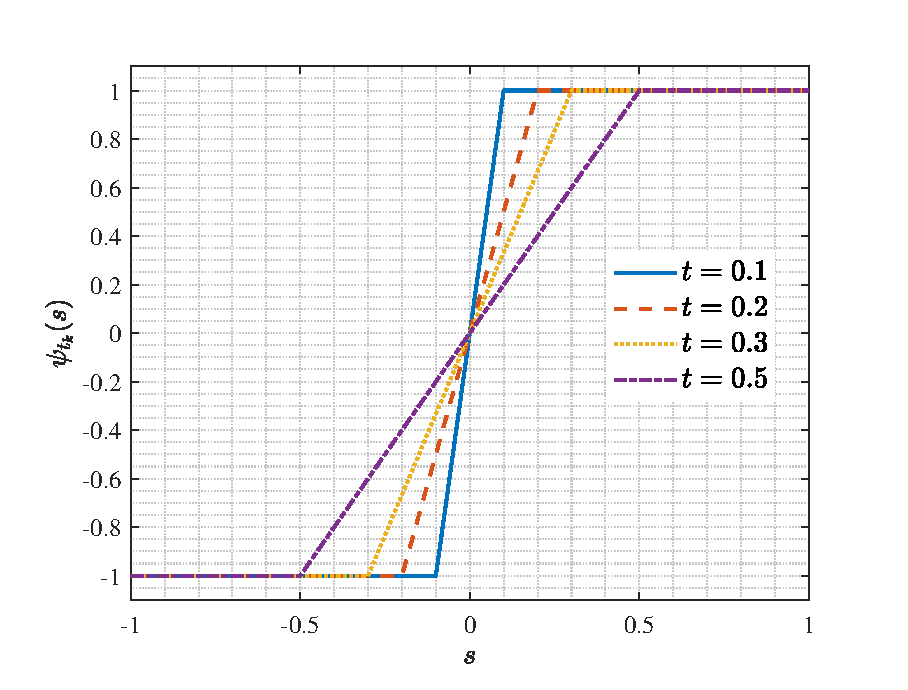
\includegraphics[width=.6\linewidth]{figures/soft_sign.eps}
    \caption{Hàm tuyến tính phân đoạn $\psi_{t_k}(s)$ được sử dụng trong DetNet.}
    \label{fig:soft_sign}
\end{figure}
Các tham số của việc học sẽ bao gồm 
\begin{equation}
\boldsymbol{\theta}=\left\{\mathbf{W}_{1 k}, \mathbf{b}_{1 k}, \mathbf{W}_{2 k}, \mathbf{b}_{2 k}, \mathbf{W}_{3 k}, \mathbf{b}_{1 k}, \mathbf{t}_k\right\}_{k=1}^K
\end{equation}

Một hàm mất mát sẽ tổng hợp sai số từ kết quả đầu ra của tất cả các lớp để ước lượng sự hội tụ của mạng DetNet. Ngoài ra, vì các lỗi ước lượng từ DetNet còn phụ thuộc vào tính ngẫu nhiên của kênh truyền nên sẽ được chuẩn hoá bằng lỗi của bộ giải mã ZF. Hàm mất mát như dưới đây
\begin{equation}
    l(\mathbf{s} ; \hat{\mathbf{s}}(\mathbf{H}, \mathbf{x}))=\sum_{k=1}^K \log (k) \frac{\left\|\mathbf{s}-\hat{\mathbf{s}}_k\right\|^2}{\|\mathbf{s}-\tilde{\mathbf{s}}\|^2}
\end{equation}
với $\tilde{\mathbf{s}}$ là ước lượng của $\mathbf{s}$ thu được từ bộ giải mã ZF như trình bày trong mục~\ref{sec:zf}. Lưu ý rằng, do $\mathbf{H}$ là ma trận của các số thực nên phép chuyển vị liên hợp phức $(.)^H$ sẽ được chuyển thành chuyển vị $(.)^\top$.
\begin{equation}
    \tilde{\mathbf{s}}=\left(\mathbf{H}^\top \mathbf{H}\right)^{-1} \mathbf{H}^\top \mathbf{x}
\end{equation}

\section{Đề xuất mạng học sâu ISD cho nhận dạng kênh truyền}

Bộ nhận dạng MMSE đã được chứng minh~\cite{Rusek2013} có thể đạt được độ chính xác tối ưu của MLE cho kênh đường lên cho các hệ mMIMO với $L/T \ge 10$.
\begin{equation}
    \hat{\mathbf{s}}_{MMSE}=\left(\mathbf{H}^\top \mathbf{H}+\frac{\sigma^2}{\mathbb{E}_\mathbf{x}} \mathbf{I}_{2T}\right)^{-1} \mathbf{H}^\top \mathbf{x}=\mathbf{P}^{-1} \mathbf{q}
\end{equation}
ký hiệu $\mathbf{G} = \mathbf{H}^\top \mathbf{H}$, $\mathbf{P} = \mathbf{H}^\top \mathbf{H}+\frac{\sigma^2}{\mathbb{E}_\mathbf{x}} \mathbf{I}_{2T}$, và $\mathbf{q} = \mathbf{H}^\top \mathbf{x}$. Tuy nhiên, độ phức tạp của việc nghịch đảo $\mathbf{P}$ là $\mathcal{O}(T^3)$, sẽ tăng nhanh khi $T$ lớn. Các thành phần đường chéo (diagonal component) của ma trận $\mathbf{P}$ tạo thành ma trận $\mathbf{D}$. Giá trị khởi tạo của $\mathbf{s}_{in}$ thu được là
\begin{equation}
    \mathbf{s}_{in}=\mathbf{D}^{-1} \mathbf{q}=\left[s_0(1), s_0(2), \ldots, s_0(2T)\right]
\end{equation}

Từ véc-tơ tín hiệu thu, tín hiệu của ăng-ten/người dùng thứ $j$ thu được bằng cách loại bỏ tạp âm từ các ăng-ten/người dùng còn lại.
\begin{equation}
    \hat{\mathbf{x}}_j=\mathbf{x}-\sum_{t=1, t \neq j}^{2T} \mathbf{h}_t s_k(t)
\end{equation}
với $\hat{\mathbf{x}}_j$ thu được, ký hiệu được gửi từ người dùng thứ $j$ được ước lượng như sau
\begin{equation}
    \begin{aligned}
        s_{k+1}(j) & =\frac{\mathbf{h}_j^\top}{\left\|\mathbf{h}_j\right\|^2} \hat{\mathbf{x}}_j \\ 
        & = s_k(j)+\frac{1}{\mathbf{G}(j, j)}\left(\mathbf{q}(j)-\sum_{t=1}^{2T} \mathbf{G}(j, t) s_k(t)\right)
    \end{aligned}
\end{equation}
trong đó, $\mathbf{h}_j$ là cột thứ $j$ của ma trận $\mathbf{H}$, $\mathbf{G}(i, j)$ là phần tử thứ $(i, j)$ của ma trận $G$, và $q(j)$ là phần tử thứ $j$ của véc-tơ $\mathbf{q}$. Véc-tơ ước lượng $\mathbf{s}$ được cập nhật như trong thuật toán~\ref{alg:cap} của thuật toán ISD đã được đề xuất trong~\cite{Mandloi2017}. 
\begin{algorithm}[ht]
    \caption{Bộ nhận dạng Iterative Sequential~\cite{Mandloi2017}.}\label{alg:cap}
    \hspace*{\algorithmicindent} \textbf{Input: $\mathbf{x}, \mathbf{H}, L, T, K, \sigma^2, \mathbb{E}_\mathbf{x}$} \\
    \hspace*{\algorithmicindent} \textbf{Output: $\mathbf{s}_{out} = \mathbf{s}^{2T}_K$} 
    \begin{algorithmic}[1]
        \State $\mathbf{G} \leftarrow \mathbf{H}^\top \mathbf{H}$
        \State $\mathbf{A} \leftarrow \mathbf{G} + \frac{\sigma^2}{\mathbb{E}_\mathbf{x}} \mathbf{I}_{2T}$
        \State $\mathbf{s}_0 \leftarrow \mathbf{s}_{in} = \mathbf{D}^{-1} \mathbf{q}$ \\
        \For{ $k=0, k < K$}
            \For{ $j=1, j \le 2T$}
                \State $s_k(j+1) \leftarrow s_k(j)+\frac{1}{\mathbf{G}(j, j)}\left(\mathbf{q}(j)-\sum_{t=1}^{2T} \mathbf{G}(j, t) s_k(t)\right)$ \\ 
                \State $\mathbf{s}_{k+1}^j \leftarrow\left[s_{k+1}(1),~\ldots, s_{k+1}(j), s_k(j+1),~\ldots, s_k(2T)\right]$
                \State $j \leftarrow j + 1$
            \EndFor
            \State $k \leftarrow k + 1$
        \EndFor
    \end{algorithmic}
\end{algorithm}

\begin{equation}
    \mathbf{e}_{k+1}=\mathbf{D}^{-1}\left(\mathbf{H}^\top \mathbf{x}-\mathbf{H}^\top \mathbf{H} \mathbf{s}_k\right)
\end{equation}

\begin{equation}
\mathbf{s}_{k+1}=\mathbf{s}_k+\mathbf{e}_{k+1}
\end{equation}

\begin{equation}
\mathbf{s}_{k+1}=\left(1-\alpha_k^2\right) \mu_k + \alpha_k^2 \mathbf{s}_k
\end{equation}

\begin{equation}
\mu_k=\mathbf{s}_k+\mathbf{e}_{k+1}+\alpha_k^1 \mathbf{e}_k
\end{equation}

\begin{equation}
\mathbf{e}_0 \leftarrow \mathbf{W}_0^2\left(\mathbf{W}_0^1 \mathbf{e}_0+\mathbf{b}_0^1\right)+\mathbf{b}_0^2
\end{equation}

\begin{figure}[ht]
    \centering
    \begin{tikzpicture}
        \node (B11) [field6, fill=red!10!white] at (0, 0) {$\mathbf{e}_0$};
        \node (B21) [below=10mm of B11, field6, fill=red!10!white] {$\mathbf{s}_0$};
        \node (B31) [below=10mm of B21, field6, fill=red!10!white] {$\mathbf{H}^\top \mathbf{H}$};
        \node (B41) [below=10mm of B31, field6, fill=red!10!white] {$\mathbf{H}^\top \mathbf{x}$};
        \node (B51) [below=10mm of B41, field6, fill=red!10!white] {$\mathbf{D}^{-1}$};

        \node (B12) [right=5mm of B11, circle, fill=blue!10!white, draw=black] {$\times$};
        \node (B13) [right=5mm of B12, circle, fill=blue!10!white, draw=black] {$+$};
        \node (B14) [right=5mm of B13, circle, fill=blue!10!white, draw=black] {$\times$};
        \node (B15) [right=5mm of B14, circle, fill=blue!10!white, draw=black] {$+$};
        \node (B16) [right=5mm of B15, circle, fill=blue!10!white, draw=black] {$\times$};
        \node (B17) [right=18mm of B16, field8, fill=green!10!white, draw=black] {$\alpha^2_0$};
        \node (B18) [right=5mm of B17, circle, fill=blue!10!white, draw=black] {$\times$};

        \node (B61) [below=4mm of B12, field8, fill=green!10!white, draw=black] {$W_{10}$};
        \node (B62) [below=4mm of B13, field8, fill=green!10!white, draw=black] {$b_{10}$};
        \node (B63) [below=4mm of B14, field8, fill=green!10!white, draw=black] {$W_{20}$};
        \node (B64) [below=4mm of B15, field8, fill=green!10!white, draw=black] {$b_{20}$};
        \node (B65) [below=4mm of B16, field8, fill=green!10!white, draw=black] {$\alpha^1_0$};

        \node (B22) [right=75mm of B21, circle, fill=blue!10!white, draw=black] {$+$};
        \node (B23) [below=12mm of B18, circle, fill=blue!10!white, draw=black] {$+$};
        \node (B24) [right=5mm of B23, circle, fill=blue!10!white, draw=black] {$\rho$};

        \node (B25) [below=4mm of B23, circle, fill=blue!10!white, draw=black] {$\times$};
        \node (B26) [below=4mm of B25, field8, fill=green!10!white, draw=black] {$1 - \alpha^2_0$};

        \node (B32) [right=5mm of B31, circle, fill=blue!10!white, draw=black] {$\times$};
        \node (B42) [right=5mm of B41, circle, fill=blue!10!white, draw=black] {$-$};
        \node (B52) [right=5mm of B51, circle, fill=blue!10!white, draw=black] {$\times$};

        \node (Phi1) [right=123mm of B21, field6, fill=red!10!white] {$\mathbf{s}_1$};
        \node (V1) [right=123mm of B51, field6, fill=red!10!white] {$\mathbf{e}_{1}$};

        \draw[arrow] (B11) -- (B12);
        \draw[arrow] (B12) -- (B13);
        \draw[arrow] (B13) -- (B14);
        \draw[arrow] (B14) -- (B15);
        \draw[arrow] (B15) -- (B16);
        \draw[arrow] (B17) -- (B18);
        
        \draw[arrow] (B61) -- (B12);
        \draw[arrow] (B62) -- (B13);
        \draw[arrow] (B63) -- (B14);
        \draw[arrow] (B64) -- (B15);
        \draw[arrow] (B65) -- (B16);

        \draw[arrow] (B21) -- (B22);
        \draw[arrow] (B31) -- (B32);
        \draw[arrow] (B41) -- (B42);
        \draw[arrow] (B51) -- (B52);
        \draw[arrow] (B52) -- (V1);

        \draw[arrow] (B18) -- (B23);
        \draw[arrow] (B23) -- (B24);
        \draw[arrow] (B24) -- (Phi1);

        \draw[arrow] (B16) -| (B22);
        \draw[arrow] (B25) -- (B23);
        \draw[arrow] (B26) -- (B25);
        \draw[line] (B22) -- ([xshift=3mm]B22.east);
        \draw[arrow] ([xshift=3mm]B22.east) |- (B25);
        \draw[line] (V1) -- ([yshift=15mm]V1.north);
        \draw[arrow] ([yshift=15mm]V1.north) -| (B22);

        \draw[arrow] (B21) -| (B32);
        \draw[arrow] (B32) -- (B42);
        \draw[arrow] (B42) -- (B52);

        \draw[line] (B21) -| ([xshift=-3mm, yshift=28mm]B21.west);
        \draw[arrow] ([xshift=-3mm, yshift=28mm]B21.west) -| (B18);

        \draw[arrow] (Phi1) -- ([xshift=3mm]Phi1.east);
        \draw[arrow] (V1) -- ([xshift=3mm]V1.east);

        % Legends
        \node[rectangle, draw=black, dashed, fill=black!5!white, minimum width=100mm, minimum height=35mm] at (70mm, -105mm) {};

        \node (B51) [field6, fill=red!10!white] at (37mm, -97mm) {Giá trị \\đầu vào/đầu ra};

        \node (B61) [below=4mm of B51, field8, fill=green!10!white, draw=black] {Giá trị học};

        \node (B52) [right=7mm of B51, circle, fill=blue!10!white, draw=black] {$\times$};
        \draw[arrow] (B52) -- ([xshift=3mm]B52.east) node [pos=0, right=3mm] {Nhân};

        \node (B53) [below=7mm of B52, circle, fill=blue!10!white, draw=black] {$+$};
        \draw[arrow] (B53) -- ([xshift=3mm]B53.east) node [pos=0, right=3mm] {Cộng};

        \node (B54) [right=20mm of B52, circle, fill=blue!10!white, draw=black] {$\rho$};
        \draw[arrow] (B54) -- ([xshift=10mm]B54.east) node [pos=0, right=10mm, above, label={below}:{tuyến tính}] {Toán tử};

        \node (B55) [right=20mm of B53, circle, fill=blue!10!white, draw=black] {$-$};
        \draw[arrow] (B55) -- ([xshift=3mm]B55.east) node [pos=0, right=3mm] {Trừ};
    \end{tikzpicture}
    \caption{Kiến trúc của lớp đầu tiên trong mô hình mạng ISD đề xuất.}
    \label{fig:ISD}
\end{figure}

\begin{figure}[ht]
    \centering
    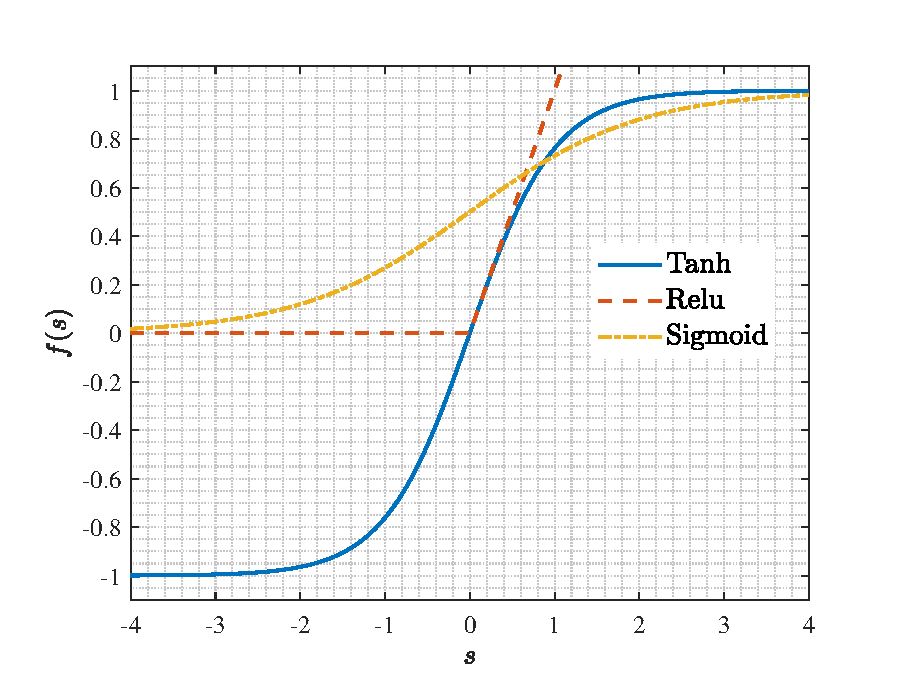
\includegraphics[width=.6\linewidth]{figures/tanh.eps}
    \caption{Minh hoạ một số hàm kích hoạt được dùng trong mô hình đề xuất.}
    \label{fig:tanh}
\end{figure}

\section{Mô phỏng và đánh giá}

\subsection{Tạo bộ dữ liệu}

\begin{table}[ht]
    \centering
    \caption{So sánh độ phức tạp của các thuật toán nhận dạng kênh truyền.}
    \label{tab:computational}
    \begin{tabular}{|l|c|c|}
    \hline
    \multicolumn{1}{|c|}{Detector} & Computational complexity & Trainable parameters \\ \hline
    ZF & $\mathcal{O}$ ($NK^3$) &  \\ \hline
    MMSE & $\mathcal{O}$ ($NK^3$) &  \\ \hline
    MLE & $\mathcal{O}$ ($NK^3$) &  \\ \hline
    DetNet~\cite{Samuel2019} & $\mathcal{O}$ ($NK^2$) & 249600 \\ \hline
    Proposed ISD & $\mathcal{O}$ ($NK^2$) & 12 \\ \hline
    \end{tabular}
\end{table}

\begin{table}
    \centering
    \caption{Các tham số mô phỏng kênh truyền vô tuyến.}
    \label{tab:simu_param}
    \begin{tabular}{p{8cm}|p{6cm}} 
    \hline
    \hline
    \multicolumn{1}{c|}{\textbf{Thông số mô phỏng}} & \multicolumn{1}{c} {\textbf{Giá trị}} \\ 
    \hline
    Kích thước hệ thống m-MIMO & $T = 8, L =64$ \\ 
    \hline
    Loại điều chế & 16-QAM\\
    \hline
    Các mức $\operatorname{SNR}$ của dataset  & $[0, 5, 10, 15, 20]$~dB \\ 
    \hline
    Số mẫu đào tạo & 50.000 \\ 
    \hline
    Số mẫu thử nghiệm & 10.000 \\ 
    \hline
    Bộ tối ưu & ADAM \\ 
    \hline
    Giá trị khởi tạo của tỷ lệ học & $\delta = 0$,$0001$ \\ 
    \hline
    Số vòng lặp đào tạo & 200.000 \\
    \hline
    \end{tabular}
\end{table}

\subsection{Đánh giá sự hội tụ của mạng ISD}

\subsection{Đánh giá mô hình được đào tạo}

\section{Kết luận chương}